\documentclass[t, notes, xcolor=table]{beamer}

\usepackage{wrapfig}
\usepackage{float}
% For tabs in verbatim
\usepackage{fancyvrb}

% Adjust position of the image
\usepackage[export]{adjustbox}

% set fonts
\usefonttheme{professionalfonts} % using non standard fonts for beamer
\usepackage{txfonts,mathptmx}

% set indend spacing for first and second level indentation
\setlength{\leftmargini}{0.5cm}
\setlength{\leftmarginii}{0.5cm}
\setlength{\leftmarginiii}{0.5cm}

% Set circles for bullets 
\setbeamertemplate{itemize items}[circle]

% colors
\usepackage{xcolor}

% multiple columns
\usepackage{multicol}

% todo lists
\usepackage{pifont}
\usepackage{amssymb}

% increase space between text and frame name
\addtobeamertemplate{frametitle}{}{\vspace{0.5em}}

%Information to be included in the title page:
\title{Using Continuous and Procedural Assignments}
\author{Nikola Petrovic}
\institute{University of Belgrade, School of Electrical Engineering}
\date{2022}



\begin{document}

\frame{\titlepage}

%%%%%%%%%%%%%%%%%%%%%%%%%%%%%%%%%%%%%%%%%%%%%%%%%%%%%%%%%%%%
\begin{frame}
\frametitle{Module Objective}

In this module we will appropriately choose between continuous and procedural assignments.
\newline

\textbf{Topics:}
\begin{itemize}
\item Continuous assignments review
\item Multiple continuous assignments to a single net
\item Procedural assignments review
\item Multiple procedural assignments to a single variable
\item Understanding the simulation cycle
\item Conditional operator revisit
\item Feedback loops
\item Generate Statements
\end{itemize}

\end{frame}
\note{
Our objective is to appropriately select between continuous and procedural statements. To do that, we need to know in more detail how these two different kinds of assignments work.

}

%%%%%%%%%%%%%%%%%%%%%%%%%%%%%%%%%%%%%%%%%%%%%%%%%%%%%%%%%%%%
\begin{frame}
\frametitle{Continuous Assignments Review}
\footnotesize{
\begin{multicols}{2}
\begin{itemize}
\item Only outside procedural blocks
\item Continuously drive nets
\item Order of declaration does not affect functionality
\end{itemize}

\vfill
\columnbreak
\begin{figure}
    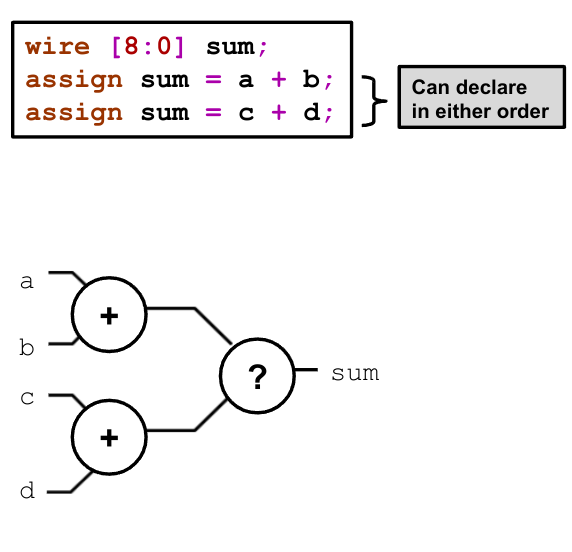
\includegraphics[width=0.45\textwidth]{img/08_cont_re.png}
\end{figure}
\end{multicols}
}
\end{frame}
\note{
\scriptsize{
A continuous assignment is its own process - the simulator automatically updates the driven value and resolved net value when any of the inputs transition.
\newline

We can place a continuous assignment in a module anywhere after we declare the primaries that are its inputs. For tools compliant with the Verilog 2005 standard, we do not need to declare the target. The target of a continuous assignment is implicitly declared as a scalar net of the default net type, usually a wire. Reliance upon implicit declarations is generally considered poor practice.
\newline

The simulator updates continuous assignments in any simulation cycle in which their inputs transition. No order is implied among multiple continuous assignments updated in the same simulation cycle. Relative position in the source code has no effect.

}
}

%%%%%%%%%%%%%%%%%%%%%%%%%%%%%%%%%%%%%%%%%%%%%%%%%%%%%%%%%%%%
\begin{frame}
\frametitle{Multiple Continuous Assignments}
\scriptsize{
\begin{multicols}{2}
Multiple continuous assignments to a single net are "wired together".
\newline

The \textcolor{purple}{wire}, \textcolor{purple}{wand} and \textcolor{purple}{wor} net types all resolve value conflicts differently.
\vfill
\columnbreak
\begin{figure}
    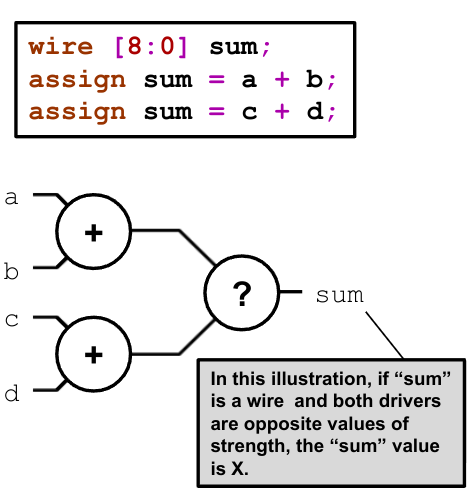
\includegraphics[width=0.4\textwidth]{img/08_cont_mult.png}
\end{figure}
\end{multicols}
}
\begin{figure}
    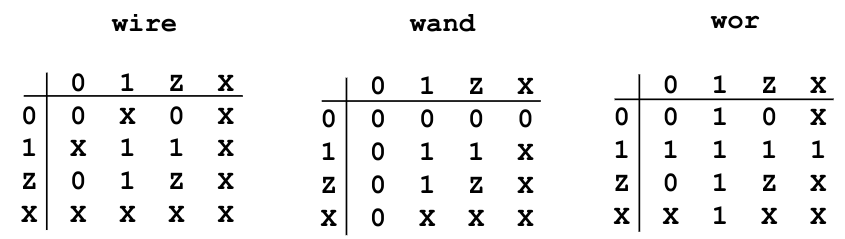
\includegraphics[width=0.75\textwidth]{img/08_cont_mult_table.png}
\end{figure}
\end{frame}
\note{
\scriptsize{
Except for the Verilog-2005 unresolved wire (\textbf{uwire}) type, the simulator resolves the value of a net driven by multiple drivers. The \textbf{uwire} type does not accept multiple drivers and reports an error.
\begin{itemize}
\item If one driver is stronger than the others, the strong driver "wins". We can, for example, pull up a wire and still drive it to the 0,1 and unknown (x) values. When we drive it to the high-impedance (z) value, the pull-up takes over to maintain a pull-strength 1 on the wire. \textit{Appendix B: Modeling with Verilog Primitives and UDPs} examines drive strengths in detail.
\item If more than one driver is equally stronger than the remaining drivers, the simulator resolves the value of a net. The resolution function depends upon the net type and is different for nets that do and do not represent wired logic.
\begin{itemize}
\scriptsize{
\item A \textbf{wire} net will attain 0 or 1 value when all such strong drivers drive either a high-impedance value or the same 0 or 1 value and none of them drive an unknown value.
\item A wired-AND (\textbf{wand}) net will attain 0 value when any such strong drivers drive a 0 value.
\item A wired-OR (\textbf{wor}) net will attain the 1 value when any such strong drivers drive a 1 value.
}
\end{itemize}
\end{itemize}

}
}

%%%%%%%%%%%%%%%%%%%%%%%%%%%%%%%%%%%%%%%%%%%%%%%%%%%%%%%%%%%%
\begin{frame}
\frametitle{Procedural Assignments Review}
\scriptsize{
\begin{multicols}{2}
\begin{itemize}
\item Procedural blocks start with \textcolor{purple}{always} or \textcolor{purple}{initial}.
\item An event control almost always immediately follows the \textcolor{purple}{always} keyword.
\begin{itemize}
	\scriptsize{
	\item Blocks further statement execution until an event occurs.
	}
\end{itemize}
\item Statements within a sequential block (\textit{begin-end}) execute sequentially.
\item Assignments are only to variables - not nets.
\item Multiple procedural blocks execute "concurrently".
\end{itemize}

\vfill
\columnbreak
\begin{figure}
    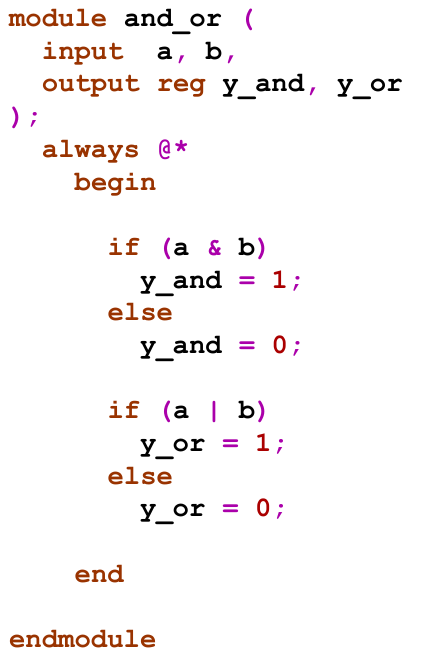
\includegraphics[width=0.4\textwidth]{img/08_proc_re.png}
\end{figure}
\end{multicols}
}
\end{frame}
\note{
\tiny{
A procedural block is a process. It reacts to input transitions and generates output transitions.
\newline

We start a procedural block with and \textbf{always} keyword or an \textbf{initial} keyword. The \textbf{always} keyword starts a block that executes continually and the \textbf{initial} keyword starts the block that executes once. We control the execution of a procedural block by using timing controls. The most common of these is the event control, which blocks further statement execution until an event occurs.
\newline

The \textbf{always} and \textbf{initial} keywords apply to a following statement. That following statements is often statement group between the \textbf{begin} and \textbf{end} keywords. Statements between \textbf{begin} and \textbf{end} words executes sequentially. The previous statement finishes execution before the next statement starts. The Verilog for Verification section in this course examines a similar construct that encloses statements executing concurrently.
\newline

The procedural assignments can be blocking assignments (=). They are called blocking assignments because they block execution of the next statement until they complete. This ensures that future statements can use the new value of the updated variable. We will often see it written that these assignments are "immediate", but that is not  true, as we will later see haw we can deliberately delay it.
\newline

Non-blocking assignments use the same token as the less-than-or-equal-to ($<$=) operator. They are called non-blocking assignments because their completion is scheduled and they do not block execution of the next statement.

}
}

%%%%%%%%%%%%%%%%%%%%%%%%%%%%%%%%%%%%%%%%%%%%%%%%%%%%%%%%%%%%
\begin{frame}
\frametitle{Multiple Procedural Assignments}
\scriptsize{
\begin{multicols}{2}
Statements within a sequential block (begin-end) executes sequentially.
\begin{itemize}
\item Subsequent assignments override previous assignments
\end{itemize}
\vfill
\columnbreak
\begin{figure}
    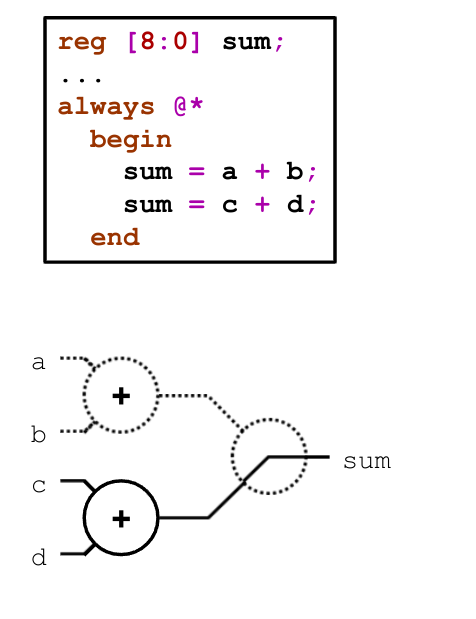
\includegraphics[width=0.45\textwidth]{img/08_proc_mult.png}
\end{figure}
\end{multicols}
}
\end{frame}
\note{
\scriptsize{
Statements within a sequential block execute sequentially. Subsequent assignments override previous assignments. The latest assignment to a variable overrides all previous assignments to the variable.
\newline

This example first assigns to the variable the sum of $a+b$. The without any delay it assigns to the variable the sum of $c+d$. The first assignment has no duration, so no other block can observe its results. No glitch will occur. Smart simulators will see this and optimize away the first assignment.

}
}
%%%%%%%%%%%%%%%%%%%%%%%%%%%%%%%%%%%%%%%%%%%%%%%%%%%%%%%%%%%%
\begin{frame}
\frametitle{Example Multiple Procedural Assignments}
\scriptsize{
\begin{multicols}{2}
\begin{itemize}
\item Subsequent assignments override previous assignments.
\item Both these code fragments are equivalent.
\item The version with the default assignment statement will be preferred for synthesis.
\end{itemize}
\vfill
\columnbreak
\begin{figure}
    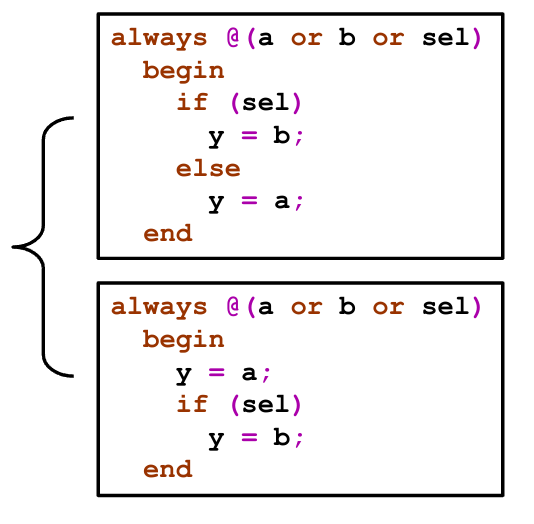
\includegraphics[width=0.45\textwidth]{img/08_proc_mult_example.png}
\end{figure}
\end{multicols}
}
\end{frame}
\note{
\scriptsize{
Statements within a sequential block execute sequentially. Subsequent assignments override previous assignments. The latest assignment to a variable overrides all previous assignments to the variable.
\newline

This semantic is quite useful. We can write a code block that first provides default values for all the variables it updates, and then executes it algorithm to conditionally update some variables with various values. Upon exiting the block, we know that it has provided values for all of its variables. none has been missed regardless of what path the execution took through the block.
\newline

This illustration replaces the default branch of an \textbf{if} statement with a default assignment. The illustration is admittedly trivial, but does serve to illustrate the concept. Imagine a larger block having a perhaps 50 statements and several possible paths through statements.

}
}

%%%%%%%%%%%%%%%%%%%%%%%%%%%%%%%%%%%%%%%%%%%%%%%%%%%%%%%%%%%%
\begin{frame}
\frametitle{Conditional Operator Revisited}
\scriptsize{
\begin{multicols}{2}
\begin{itemize}
\item Can replace a simple combinational procedure with a continuous assignment.
\item Target must be a net!
\item Event control is assumed.
\item May be more "readable" than procedural equivalent.
\end{itemize}

\vfill
Both modules are equivalent.
\columnbreak
\begin{figure}
    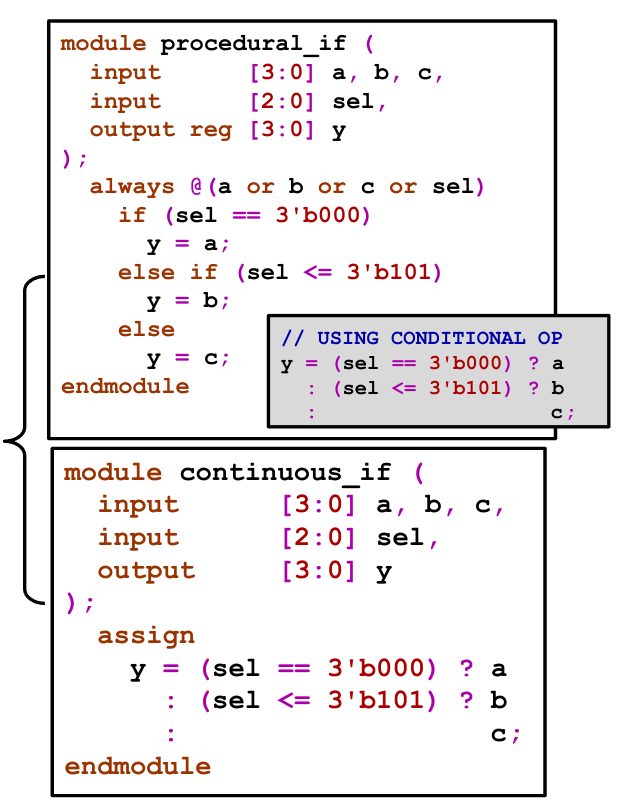
\includegraphics[width=0.5\textwidth]{img/08_cond_op.png}
\end{figure}
\end{multicols}
}
\end{frame}
\note{
\scriptsize{
For assignments to a single target, a conditional operator may be more readable than a conditional statement, and with the conditional operator, we can alternatively make the assignment a continuous assignment instead of a procedural assignment. Remember that continuous assignments are to nets and procedural assignments are to variables.

}
}

%%%%%%%%%%%%%%%%%%%%%%%%%%%%%%%%%%%%%%%%%%%%%%%%%%%%%%%%%%%%
\begin{frame}
\frametitle{Combinational Feedback Loops - Be Careful}
\scriptsize{
\begin{multicols}{2}
Zero-delay feedback loops may cause the simulator to appear to "lock up".
\begin{itemize}
\item The process never finishes or suspends.
\item The simulator never gets to do anything else.
\end{itemize}
Here is a short feedback loop deliberately generating a clock:
\begin{itemize}
\item For illustrative purposes only - more elegant ways exist to generate a clock.
\item A continuous assignment is its own process. Whenever clk\_out changes, the value is updated continuously.
\end{itemize}
\vfill
\columnbreak
\begin{figure}
    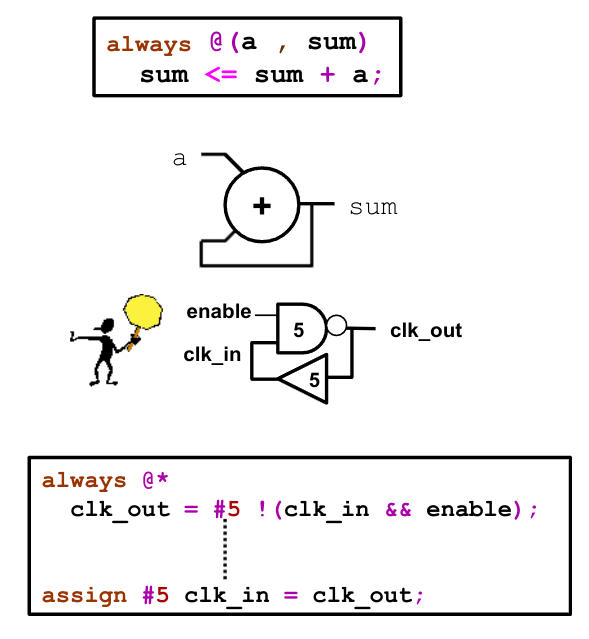
\includegraphics[width=0.45\textwidth]{img/08_feedback_loop.png}
\end{figure}
\end{multicols}
}
\end{frame}
\note{
\scriptsize{
The semantics of a Verilog process is that it reacts to its inputs and generates outputs. This is a different semantic than a procedural programming language such as C that does not autonomously react to inputs.
\newline

In continuous assignments, the simulator automatically updates the driven value and resolved net value when any of the inputs transition. For this illustration, the process is sensitive to its output, so the simulator could enter a tight loop where it does nothing but continually update the net.
\newline

We may understand this behaviour better by instead making a procedural assignment to a variable within an always block and triggering the assignment with the same set of events. The assignment occurs when any of the inputs transition, so again the simulator could enter a tight loop where it does nothing but continuously update the variable.

}
}

%%%%%%%%%%%%%%%%%%%%%%%%%%%%%%%%%%%%%%%%%%%%%%%%%%%%%%%%%%%%
\begin{frame}
\frametitle{Generate Statements in Verilog-2001}
\scriptsize{
Verilog 2001 adds new reserved keywords: \textcolor{purple}{generate endgenerate genvar}
\begin{itemize}
\item Defined within a module
\item Used to generate code dynamically within a module using conditional statements
\item \textcolor{purple}{genvar} is a positive integer value, used only inside a generate block
\item Generate\_block\_name (optional) is used to create an unique instance name for each generated item
\item Conditional (\textbf{case}, \textbf{if}) generation
\begin{itemize}
\scriptsize{
	\item Instances, functions, tasks, variables, and procedural blocks
}
\end{itemize}
\item Iterative (\textbf{for}) generation
\begin{itemize}
\scriptsize{
	\item Instances, variables and procedural blocks (no functions and tasks)
}
\end{itemize}
\item The keywords \textcolor{purple}{generate-endgenerate} are optional in Verilog-2005
\end{itemize}
}
\end{frame}
\note{
\scriptsize{
Place our generated instances, functions, tasks , variables, and procedural blocks between the \textbf{generate} and \textbf{endgenerate} reserved words ( we may not include parameters, ports, or specify blocks).
\newline

Declare \textbf{genvar} index variables for our generate \textbf{for} loops. We can declare them either inside or outside the \textit{generate} statement. We can assign only integer values to them, and only within a \textit{for} loop. These variables disappear after elaboration and are not available during simulation.
\newline

Iteratively generate statements using the \textit{for} construct. Declare a named block within the \textit{for} construct - this becomes the name of an array of scopes to match the iterations of the \textit{for} construct. Inside this named block place our generated instances, variables and procedural blocks. (We cannot define tasks and functions within a generate \textit{for} construct.)
\newline

Conditionally generate statements using the \textbf{case} and \textbf{if} constructs.


}
}

%%%%%%%%%%%%%%%%%%%%%%%%%%%%%%%%%%%%%%%%%%%%%%%%%%%%%%%%%%%%
\begin{frame}
\frametitle{Generate Statement - Conditional if Example}
\begin{itemize}
\item Conditional \textit{if} generation:
\begin{itemize}
	\item Instances, functions, tasks, variables and procedural blocks
\end{itemize}
\item Label not required to create generate-if scope.
\end{itemize}
\begin{figure}
    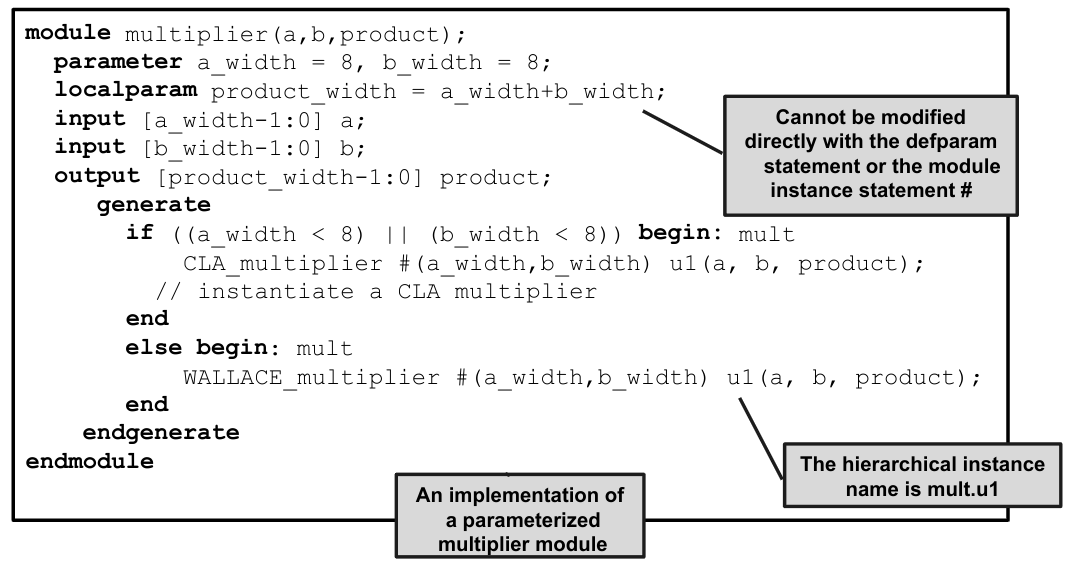
\includegraphics[width=0.95\textwidth]{img/08_gen_if.png}
\end{figure}
\end{frame}
\note{
\scriptsize{
These are the examples for usage of the \textit{generate} statement using the conditionals \textit{if-else}, case and for iterative \textit{for}.
\newline

A \textit{generate-for} loop permits one or more generate items to be instantiated multiple times. The index loop variable must be \textbf{genvar}. This example shows a parametrized gray-code to binary-code converter using a loop to generate a continuous assignment for each bit of the converter.
\newline

A \textit{generate if-else} or case permits generate items to be conditionally instantiated based on an expression that is deterministic at the time the design is elaborated.
\newline

The \textit{if-else} generate example shows the generation of instances of a carry-look-ahead multiplier. If the input bus widths are greater that 8 bits, then an instance of a wallace-tree multiplier is generated.

}
}

%%%%%%%%%%%%%%%%%%%%%%%%%%%%%%%%%%%%%%%%%%%%%%%%%%%%%%%%%%%%
\begin{frame}
\frametitle{Generate Statement - Conditional case Example}
\begin{itemize}
\item Conditional case generation
\begin{itemize}
	\item instances, functions, tasks, variables and procedural blocks
\end{itemize}
\item Label not required to create \textit{generate-case} scope.
\end{itemize}
\begin{figure}
    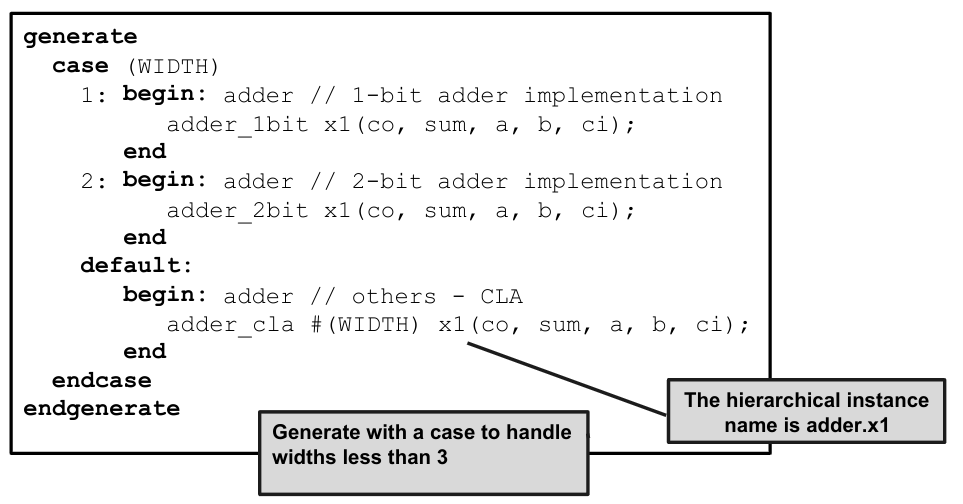
\includegraphics[width=0.95\textwidth]{img/08_gen_case.png}
\end{figure}
\end{frame}
\note{
The \textit{case-generate} example shows the instantiation of an appropriate adder depending on the case index WIDTH given as \textit{genvar}.

}

%%%%%%%%%%%%%%%%%%%%%%%%%%%%%%%%%%%%%%%%%%%%%%%%%%%%%%%%%%%%
\begin{frame}
\frametitle{Generate Statement - Iterative Example}
\begin{itemize}
\item Iterative (for) generation
\begin{itemize}
	\item Instances, variables and procedural blocks (no tasks or functions)
\end{itemize}
\item Label is required to create \textit{generate-for} scope
\end{itemize}
\begin{figure}
    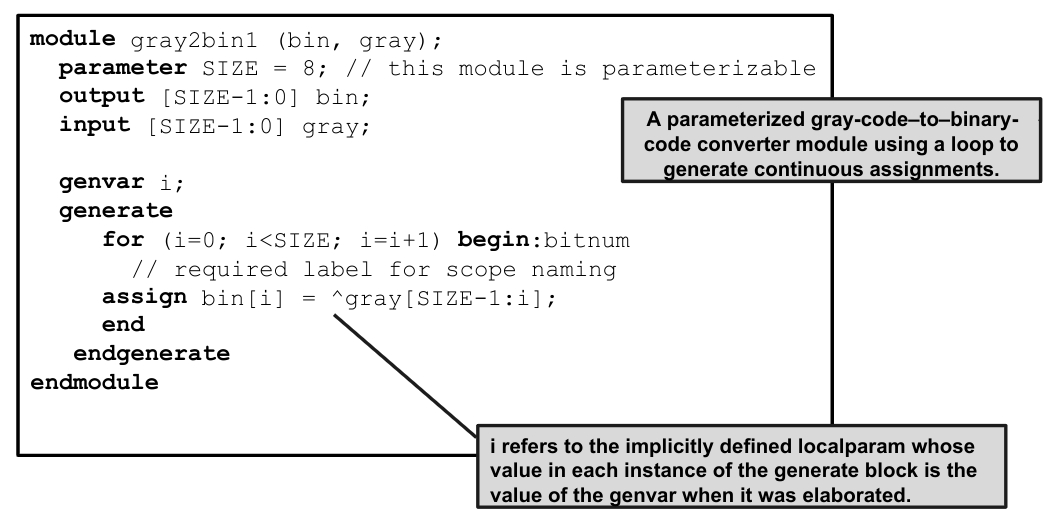
\includegraphics[width=0.95\textwidth]{img/08_gen_for.png}
\end{figure}
\end{frame}
\note{
\scriptsize{
A \textit{generate-for} loop permits one or more generate items to be instantiated multiple times. The index loop variable must be a \textit{genvar}. This example shows a parametrized gray-code to binary-code converter using a loop to generate continuous assignment for each bit of the converter.


}
}

%%%%%%%%%%%%%%%%%%%%%%%%%%%%%%%%%%%%%%%%%%%%%%%%%%%%%%%%%%%%
\begin{frame}
\frametitle{Module Summary}
\scriptsize{
Now we can appropriately choose between continuous and procedural assignments.
\newline

This module describes:
\begin{itemize}
\item Continuous assignments using \textbf{assign} that we can make only to a \textit{net} and only \textit{outside} procedural blocks. The simulator resolves a net value due to multiple continuous assignments.
\item Procedural assignments using \textbf{=} that we can make only to a \textit{variable} and only \textit{inside} procedural blocks. The last such assignment "wins" (which makes multiple such assignments in different procedural blocks problematic!)
\item The conditional operator \textbf{?:}, which is useful in both continuous and procedural assignments.
\item Inadvertently coding combinational feedback loops.
\item The generate statements introduction: Verilog-2001 construct
\end{itemize}
}
\end{frame}
\note{
We should now be able to appropriately select between continuous and procedural statements. This module described in more detail the difference between continuous statements and procedural statements.

}

%%%%%%%%%%%%%%%%%%%%%%%%%%%%%%%%%%%%%%%%%%%%%%%%%%%%%%%%%%%%
\begin{frame}
\frametitle{Module Review}
\begin{enumerate}
\item What is the result of multiple continuous assignments to a net?
\item What is the result of multiple procedural assignments to a variable?
\item Explain how the conditional operator contributes to the usefulness of continuous assignments.
\item What causes combinational feedback loops?
\end{enumerate}
\end{frame}
\note{
\scriptsize{
\begin{enumerate}
\item What is the result of multiple continuous assignments to a net?
\begin{itemize}
\scriptsize{
	\item Verilog resolves the value of multiple drivers of a net.
}
\end{itemize}
\item What is the result of multiple procedural assignments to a variable?
\begin{itemize}
\scriptsize{
	\item The last procedural assignment to the variable "wins"
}
\end{itemize}
\item Explain how the conditional operator contributes to the usefulness of continuous assignments.
\begin{itemize}
\scriptsize{
	\item A continuous assignment can sometimes more intuitively describe simple combinational logic than can a procedure. With the conditional operator, we can concisely describe more complex logic.
}
\end{itemize}
\item What causes combinational feedback loops?
\begin{itemize}
\scriptsize{
	\item A combinational feedback loop occurs when a transition on the output of a process propagates to an input of the process. A combinational loop is not a digital construct, so is a coding error in a digital design.
}
\end{itemize}
\end{enumerate}

}
}

%%%%%%%%%%%%%%%%%%%%%%%%%%%%%%%%%%%%%%%%%%%%%%%%%%%%%%%%%%%%
\begin{frame}
\frametitle{Module Exercise}
Code the following logic using a conditional operator in a:
\begin{enumerate}
\item continuous assignment
\item procedural assignment
\end{enumerate}
\begin{figure}
    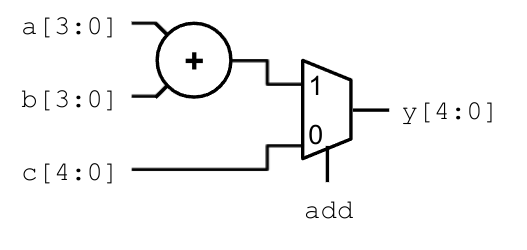
\includegraphics[width=0.55\textwidth]{img/08_ex.png}
\end{figure}
\end{frame}
\note{
Solution:

\begin{figure}
    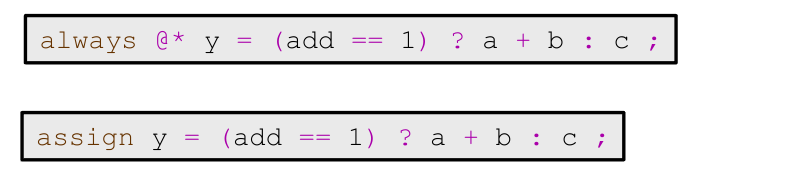
\includegraphics[width=0.55\textwidth]{img/08_ex_sol.png}
\end{figure}
}

%%%%%%%%%%%%%%%%%%%%%%%%%%%%%%%%%%%%%%%%%%%%%%%%%%%%%%%%%%%%
\begin{frame}
\frametitle{Lab}
Lab 9-1 Modeling a Single-Bidirectional-Port memory
\begin{itemize}
\item Use continuous and procedural assignments while describing a memory.
\end{itemize}
\begin{figure}
    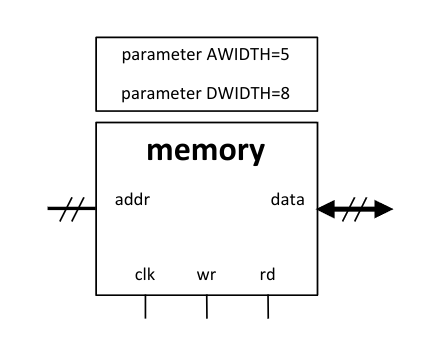
\includegraphics[width=0.45\textwidth]{img/08_lab.png}
\end{figure}
\end{frame}

%%%%%%%%%%%%%%%%%%%%%%%%%%%%%%%%%%%%%%%%%%%%%%%%%%%%%%%%%%%%
\begin{frame}[fragile]
\frametitle{Test Your Understanding - 1}

We coded the two continuous assignments to the wire \textbf{w}. At some point during simulation, \textbf{s1} and \textbf{s2} are both true. The sample code is:
\begin{Verbatim}[commandchars=\\\{\}, tabsize=2]
\textcolor{purple}{wire} w;
\textcolor{purple}{assign} w = s1 ? 1'b1 : 1'bz;
\textcolor{purple}{assign} w = s2 ? 1'b0 : 1'bz;
\end{Verbatim}
At that point the value \textbf{w} becomes:
\begin{itemize}
\item[$\square$] 1'bz
\item[$\square$] either 1'b0 or 1'b1
\item[$\square$] 1'b0
\item[$\square$] 1'bx
\item[$\square$] 1'b1
\end{itemize}
\end{frame}
\note{
\scriptsize{
We coded the two continuous assignments to the wire \textbf{w}. At some point during simulation, \textbf{s1} and \textbf{s2} are both true. The sample code is:
\newline

\textcolor{purple}{wire} w;

\textcolor{purple}{assign} w = s1 ? 1'b1 : 1'bz;

\textcolor{purple}{assign} w = s2 ? 1'b0 : 1'bz;
\newline

At that point the value \textbf{w} becomes:
\begin{itemize}
\item[$\square$] 1'bz
\item[$\square$] either 1'b0 or 1'b1
\item[$\square$] 1'b0
\item[$\boxtimes$] 1'bx
\item[$\square$] 1'b1
\end{itemize}

}
}

%%%%%%%%%%%%%%%%%%%%%%%%%%%%%%%%%%%%%%%%%%%%%%%%%%%%%%%%%%%%
\begin{frame}[fragile]
\frametitle{Test Your Understanding - 2}
We coded the two procedural assignments to the reg \textbf{r}. At some point during simulation, \textbf{s1} and \textbf{s2} are both true. The sample code is:
\begin{Verbatim}[commandchars=\\\{\}, tabsize=2]
\textcolor{purple}{reg} r;
\textcolor{purple}{always} @* r = s1 ? 1'b1 : 1'bz;
\textcolor{purple}{always} @* r = s2 ? 1'b0 : 1'bz;
\end{Verbatim}
At that point the value \textbf{r} becomes:
\begin{itemize}
\item[$\square$] 1'bz
\item[$\square$] either 1'b0 or 1'b1
\item[$\square$] 1'b0
\item[$\square$] 1'bx
\item[$\square$] 1'b1
\end{itemize}
\end{frame}
\note{
\scriptsize{
We coded the two procedural assignments to the reg \textbf{r}. At some point during simulation, \textbf{s1} and \textbf{s2} are both true. The sample code is:
\newline 

\textcolor{purple}{reg} r;

\textcolor{purple}{always} @* r = s1 ? 1'b1 : 1'bz;

\textcolor{purple}{always} @* r = s2 ? 1'b0 : 1'bz;
\newline

At that point the value \textbf{r} becomes:
\begin{itemize}
\item[$\square$] 1'bz
\item[$\boxtimes$] either 1'b0 or 1'b1
\item[$\square$] 1'b0
\item[$\square$] 1'bx
\item[$\square$] 1'b1
\end{itemize}

}
}



\end{document}
